\graphicspath{{Chapters/CrossSection/Figures/}}
\chapter{Observed Events and Cross Section Measurement}
\label{chap:CrossSection}

\section{Observed Events}

\begin{table}
\centering
  \begin{tabular}{lcccc}
    \hline\hline
     7~\tev\             & \eeee & \mmmm & \eemm & \llll \\
     \hline
Observed \ZZ\ & 16 & 23 & 27 & 66 \\
Observed \ZZs\ & 21 & 30 & 33 & 84 \\
     \hline
Expected \ZZ\ signal &   10.3 $\pm$ 0.1 $\pm$ 1.0 &  16.5 $\pm$ 0.2 $\pm$ 0.9 &  26.7 $\pm$ 0.2 $\pm$ 1.7 &  53.4 $\pm$ 0.3 $\pm$ 3.2 \\
Expected \ZZs\ signal &  12.3 $\pm$ 0.2 $\pm$ 1.2 &  20.5 $\pm$ 0.2 $\pm$ 1.1 &  31.6 $\pm$ 0.3 $\pm$ 2.0 &  64.4 $\pm$ 0.4 $\pm$ 4.0 \\
\hline
Expected \ZZ\ background  & 0.5 $\pm$ 0.6 $\pm$ 0.3 & $<0.6$ & 0.7 $\pm$ 0.7 $\pm$ 0.6 & 0.9 $\pm$ 1.1 $\pm$ 0.7 \\
Expected \ZZs\ background & 4.3 $\pm$ 1.4 $\pm$ 0.6 & $<0.9$ & 5.8 $\pm$ 1.6 $\pm$ 0.9 & 9.1 $\pm$ 2.3 $\pm$ 1.3 \\
    \hline\hline
  \end{tabular}

  \caption{\label{tab:selected_data_MC}
           Summary of observed \ZZllll and \ZZsllll\ candidates in the data, total background estimates and expected signal
       for the individual decay modes (columns 2 to 4) and for their combination (last column).
       The quoted uncertainties and limits represent 68\% confidence intervals; the first uncertainty is statistical
           while the second is systematic. The uncertainty on the
       integrated luminosity (3.9\%) % and the theoretical uncertainties on the \ZZ cross section 
       is not included. %Contributions from a Higgs boson are not included in
       %the expected signal. 
          }
\end{table}

\subsection{Kinematic Distributions}

% 7 TeV, ZZ, ZZ_pt / ZZ_m
\begin{figure}[htbp]
\begin{center}
 \subfigure[]{
 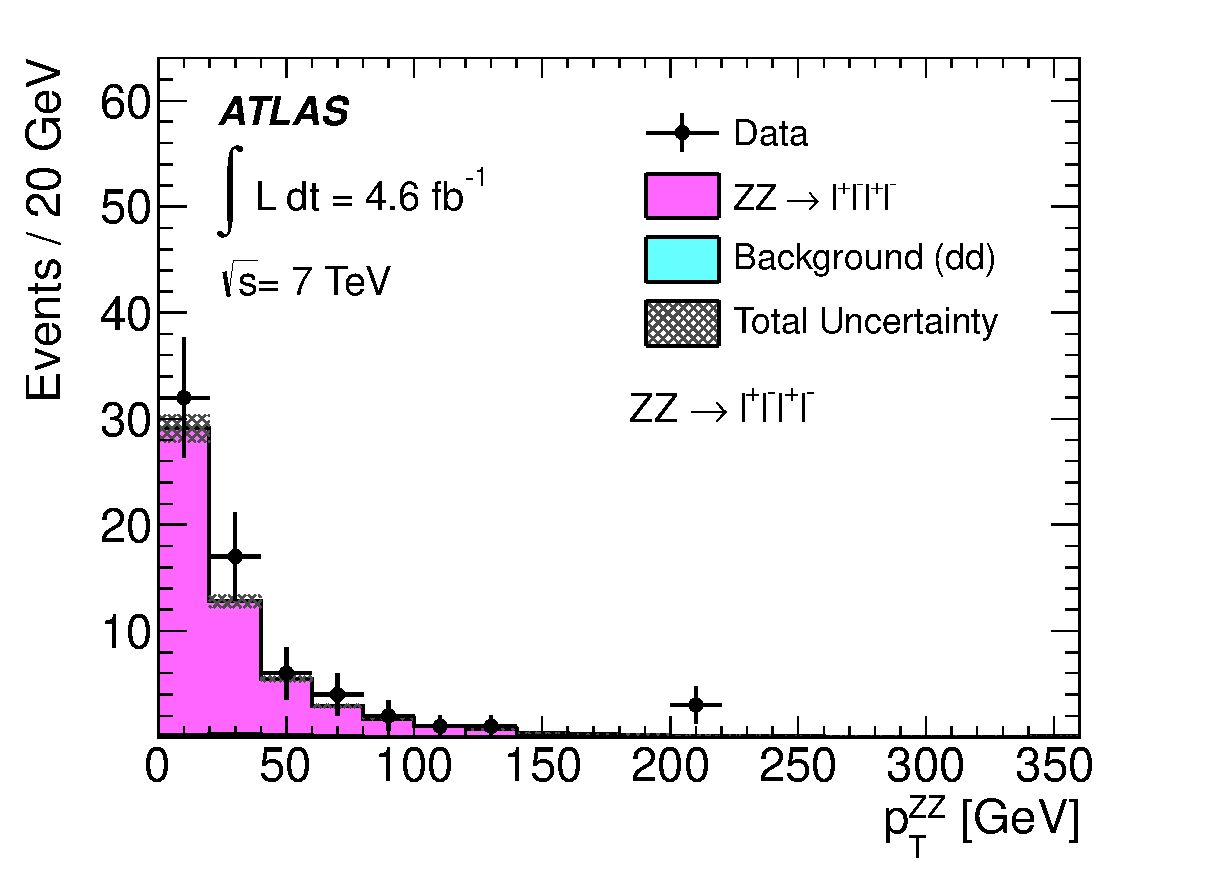
\includegraphics[width=0.47\textwidth]{7TeV/h_4l_ZZ_ZZ_pt}
 }
 \subfigure[]{
 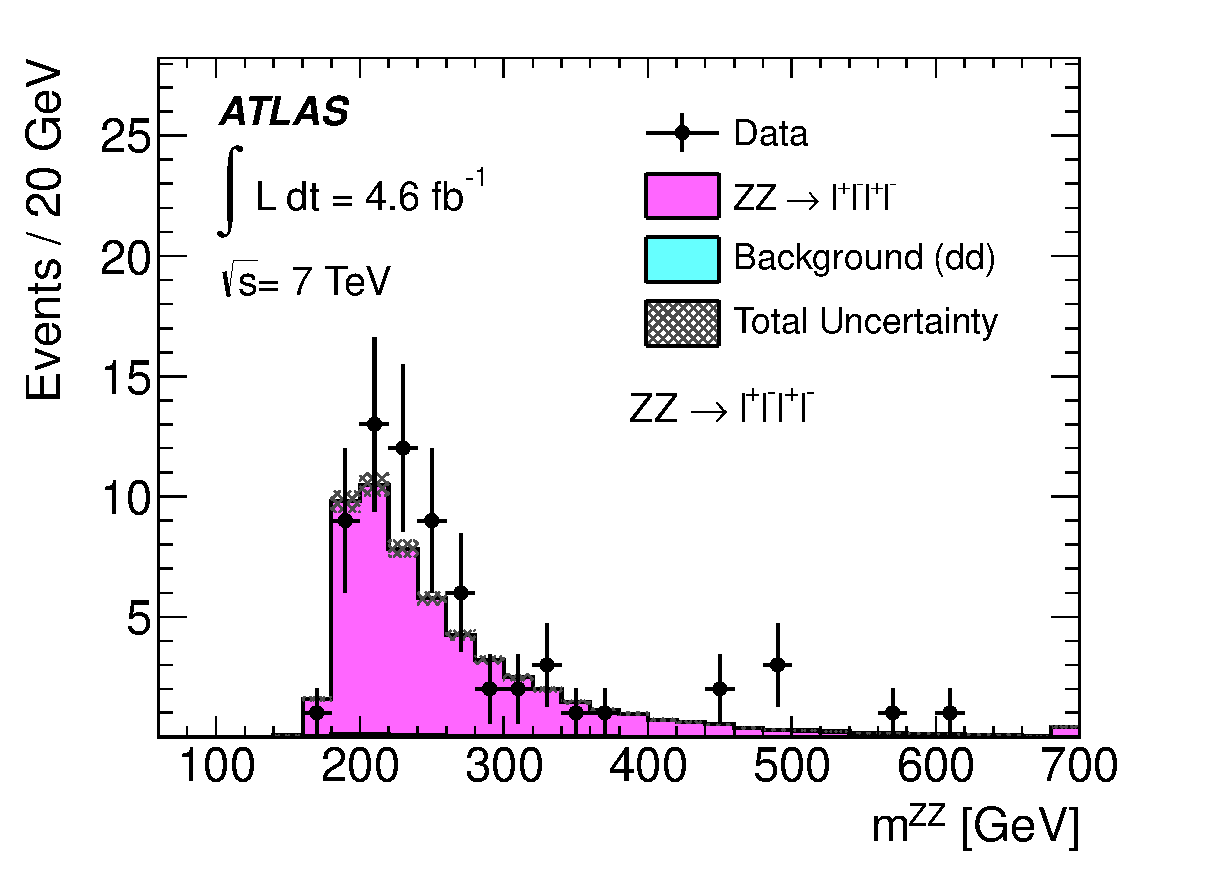
\includegraphics[width=0.47\textwidth]{7TeV/h_4l_ZZ_ZZ_m}
 }
\caption{\label{fig:kindists_zz}(a) Transverse momentum $\pT^{\ZZ}$ and (b) invariant mass $m^{\ZZ}$ of the 
           four-lepton system for the $ZZ$ selection. The points represent the observed data and the 
           histograms show the prediction from simulation, where the background
           is normalized to the data-driven (dd) estimate as described in section~\ref{sec:Background4l}. The shaded band 
           shows the combined statistical and systematic uncertainty on the prediction. 
}
\end{center}
\end{figure}

% 7 TeV, ZZ*, ZZ_pt / ZZ_m
\begin{figure}[htbp]
 \begin{center}
 \subfigure[]{
 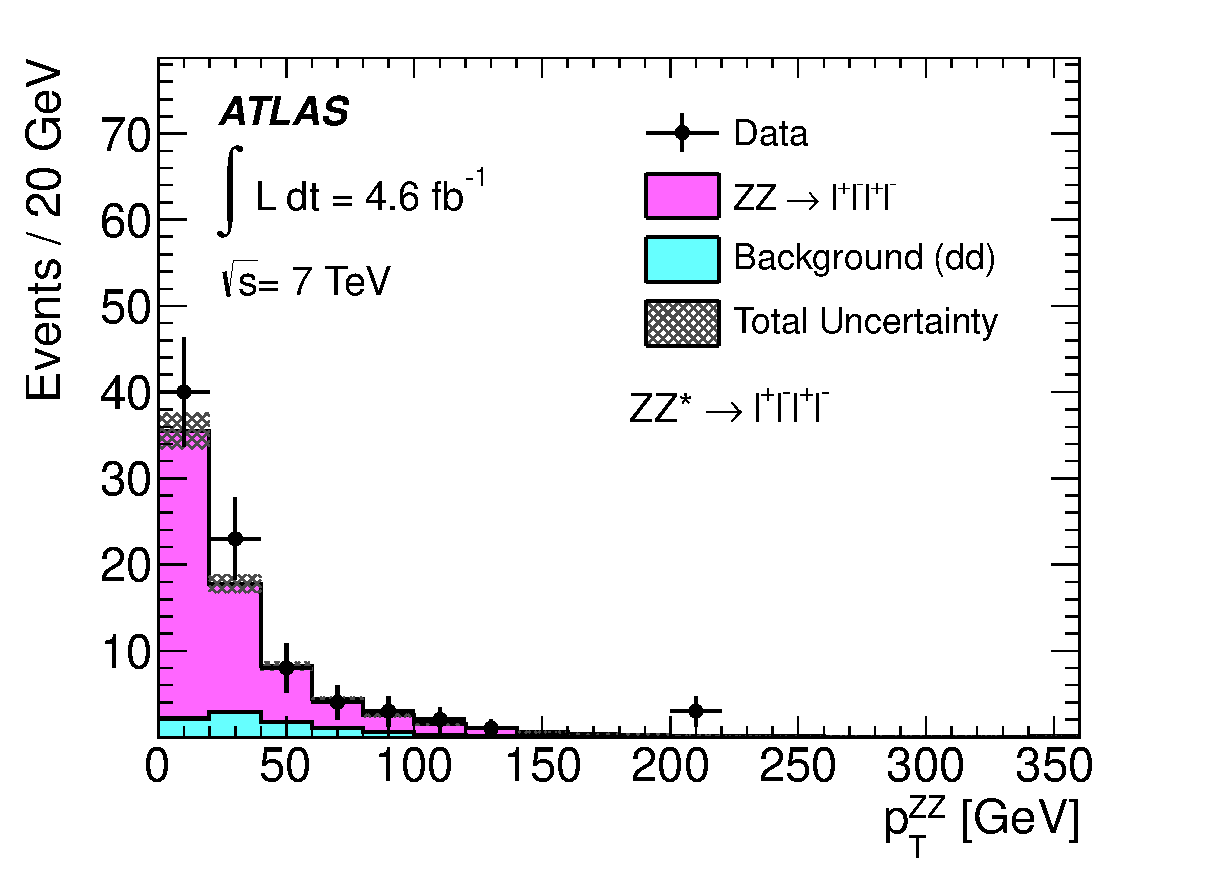
\includegraphics[width=0.47\textwidth]{7TeV/h_4l_ZZs_ZZ_pt}
 }
 \subfigure[]{
 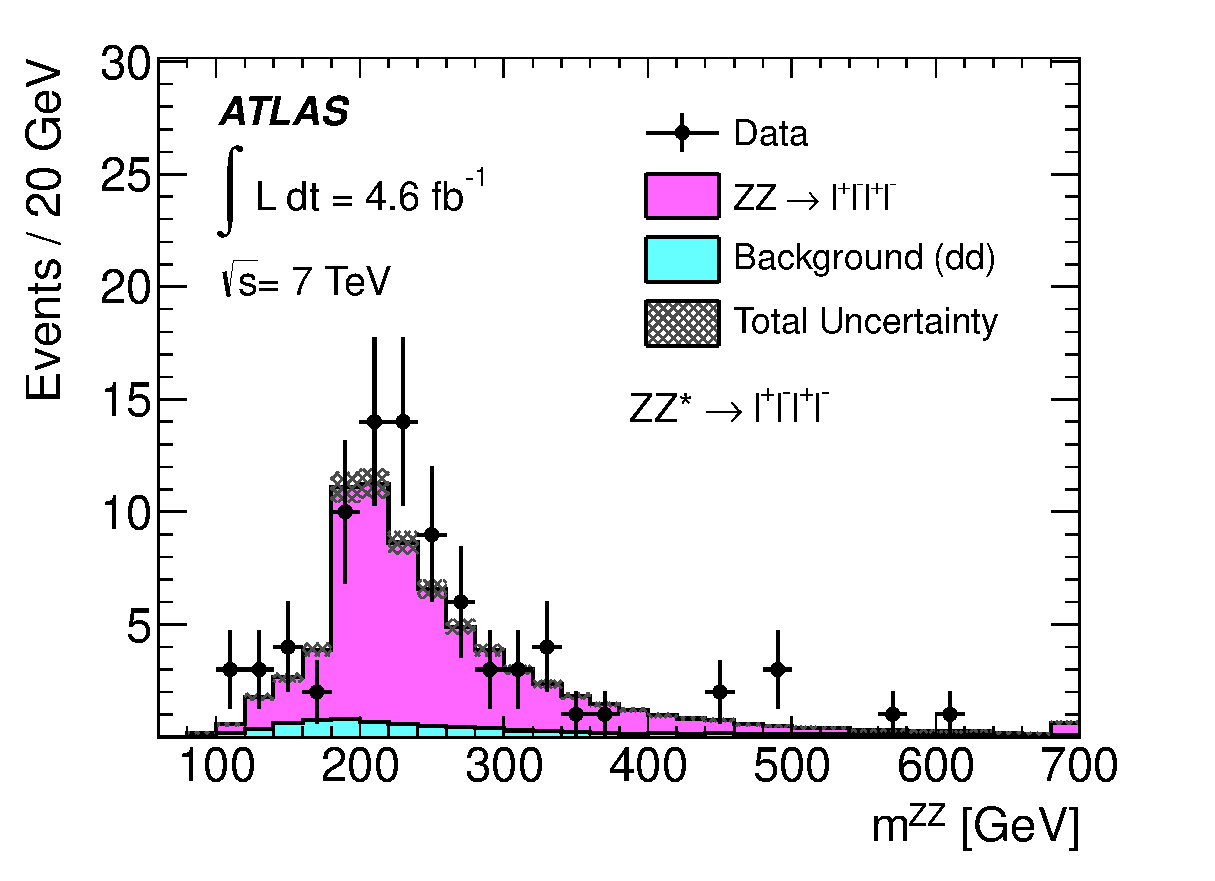
\includegraphics[width=0.47\textwidth]{7TeV/h_4l_ZZs_ZZ_m}
 }
\caption{\label{fig:kindists_zzs}(a) Transverse momentum $\pT^{\ZZ}$ and (b) invariant mass $m^{\ZZ}$ of the
           four-lepton system for the $ZZ^{*}$ selection. The points represent the observed data and the 
           histograms show the prediction from simulation, where the background
           is normalized to the data-driven (dd) estimate. 
           %as described in section~\ref{sec:Background4l}. 
           The shaded band 
           shows the combined statistical and systematic uncertainty on the prediction. 
}
\end{center}
\end{figure}

\section{Cross Section Measurement}
\subsection{Cross Section Definition}
\subsection{Fiducial Acceptance}
\subsection{Cross Section Extraction}
